\documentclass{article}
\usepackage{graphicx} % Required for inserting images
\usepackage{amsmath, amssymb, booktabs}
\usepackage{hyperref}
\usepackage{comment}

\title{Two for Two: Team Essay 2 Group 2}
\author{Jonathan Ferdinand, Devina Gera, Archimedes Li, Henry Liu, \\Katherine Shi, Sam Stevens}
\date{March 2025}

\begin{document}

\maketitle

All code can be found on our Github repository at \url{https://github.com/mshki/math-456/tree/main/essay_2}, or in Appendix A

\section{Introduction}

Our model is a multiple linear regression model that predicts the number of sales a product would get based on budgets for various methods of advertising.  Multiple linear regression is a function of multiple features, $X_1, X_2$, that predicts a label $\hat{y}$ in the form of $\hat{y} = \beta_1X_1 +\beta_2X_2 + \beta_0$.  The benefits of using a linear regression are its simplicity and high level of explainability.  This makes it a good candidate for modeling a simple relationship between variables.  However, a drawback to linear regressions is their low complexity.  We selected a dataset that fits these constraints. \\

\noindent The R packages that we used were \texttt{tidyverse} and \texttt{ggpubr} for data visualization, \texttt{lmtest} for linear regression diagnostics, \texttt{caret} for linear regression training, and \texttt{caTools} for data analysis and manipulation.

\section{Data Description}
We used the \texttt{Advertising.csv} dataset from Trevor Hastie’s “An Introduction to Statistical Learning”  GitHub page\footnote{https://trevorhastie.github.io/ISLR/Advertising.csv}. The data contains two-hundred samples of advertised products and three features (\texttt{TV}, \texttt{radio}, and \texttt{newspaper}) and one variable (\texttt{sales}) for each product. Variables \texttt{TV}, \texttt{radio}, and \texttt{newspaper} indicates the amount spent on the advertising budget for TV, radio, and newspaper, respectively, and \texttt{sales} indicates the number of sales of the product\footnote{https://search.r-project.org/CRAN/refmans/glmtoolbox/html/advertising.html}. \texttt{TV} and \texttt{radio} areslightly skew right, while (\texttt{sales} is normally distributed.   \texttt{newspaper}) is extremely skew right.

\begin{figure}[h]
    \centering
    \includegraphics[width=1\linewidth]{images/histograms.png}
    \caption{Histograms representing the frequency of different data values for each independent variable}
    \label{fig:enter-label}
\end{figure}

We can see from figure $1$ that the \texttt{newspaper} column clearly has an outlier in the histogram, which we remove.  The data adequately passed all our tests of linearity (See Analysis Section), so no additional pruning was necessary.

\section{Analysis}

We used 80\% of our  data to train the model and the remaining 20\% was used to test the model.  We used the training set to train a multiple linear regression model with TV and radio as predictors, and sales as the output.  We created a diagonal plot of this model (figure 2), which somewhat satisfies the linearity constraints.

\begin{figure}[h]
    \centering
    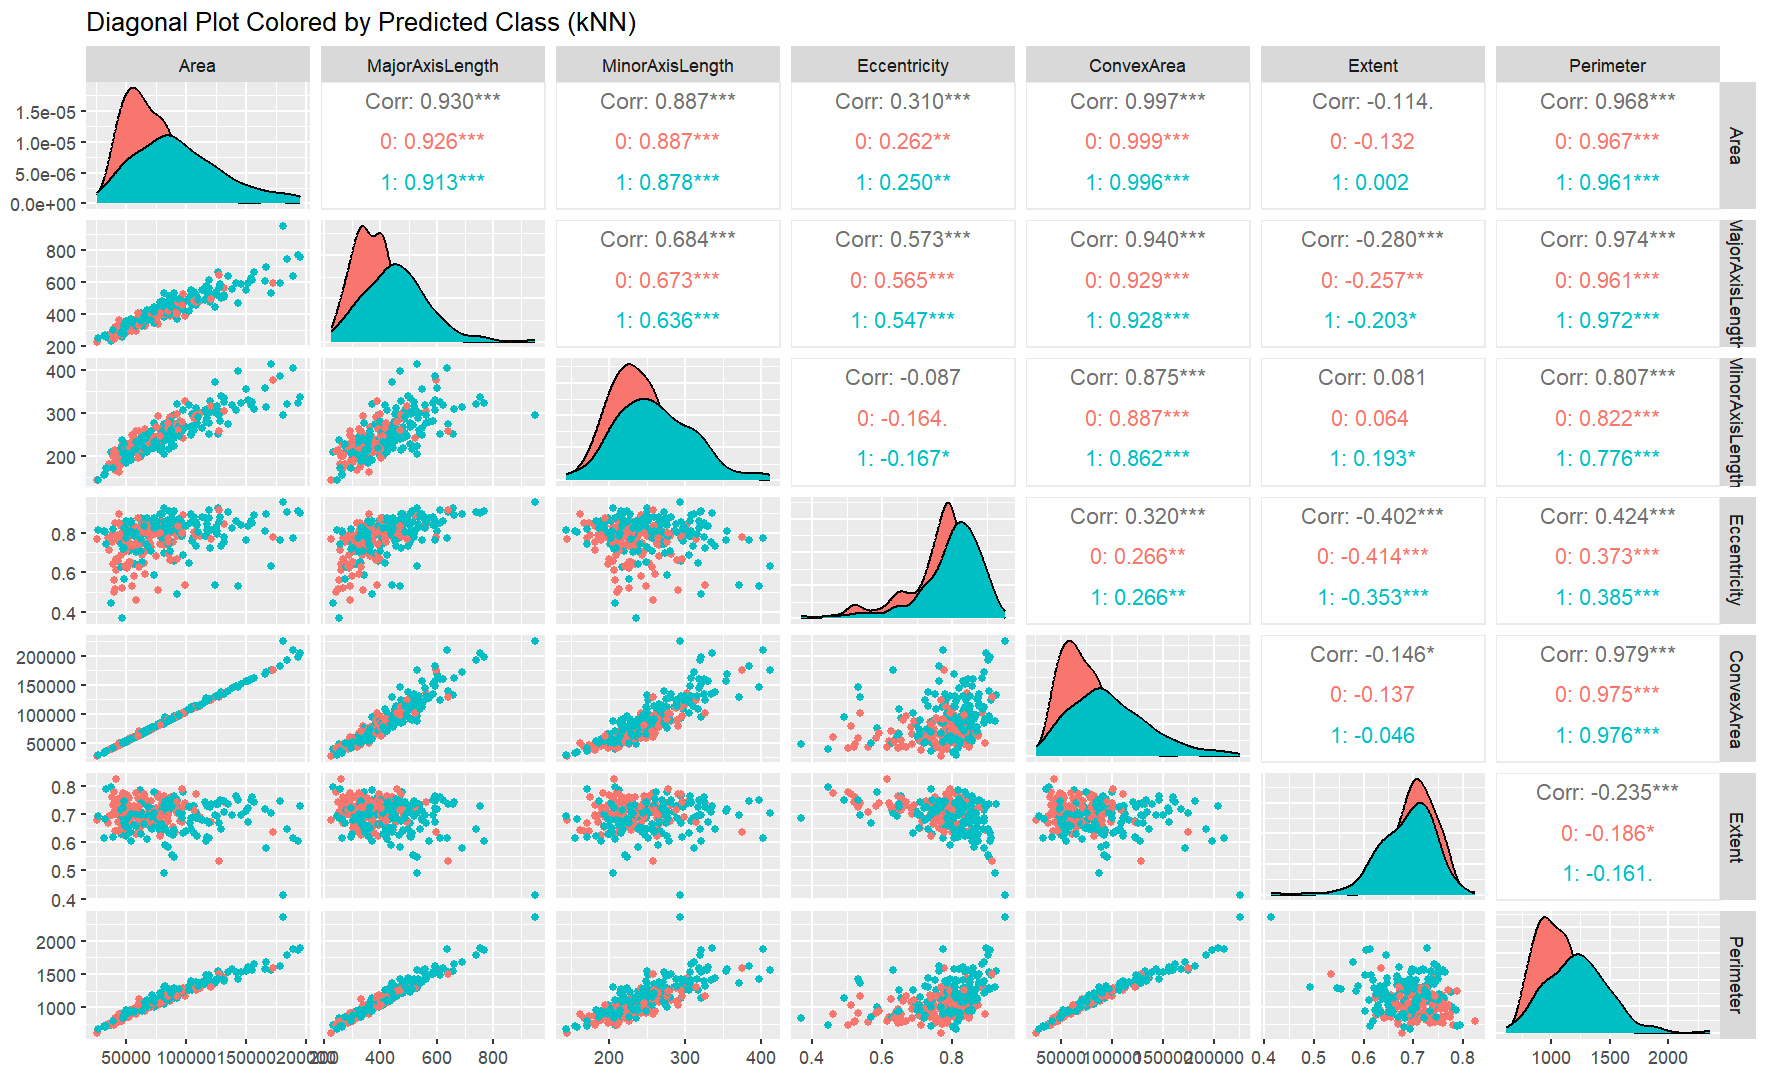
\includegraphics[width=0.9\linewidth]{images/diagonal.png}
    \caption{Diagonal plots demonstrating validity of assumptions needed for linear model}
    \label{fig:enter-label}
\end{figure}

The residuals have approximately mean zero, which satisfies our linearity assumption. The Durbin Watson test gives us a P value of 0.71, which is greater than 0.05, so we fail to reject the null hypothesis that the predictors are linearly independent. This is also supported by figure 3, which shows low correlation between predictors. The residuals vs fitted plot shows that the linear model doesn’t fully represent the relationship between advertising budget (TV, radio) and sales. The residual errors also do not have a mean value of zero. The residual errors have approximately constant variance, since the scale-location plot does not exhibit any patterns.  The Q-Q residuals show a very slight non-linear pattern, which means our assumption of normal residuals is not completely correct, but very close. The residuals vs leverage plot shows points with higher leverage also have high residuals which is not good for our model because the high influence points do not fit the model well and have high impact on the model. 

\begin{figure}[h!]
    \centering
    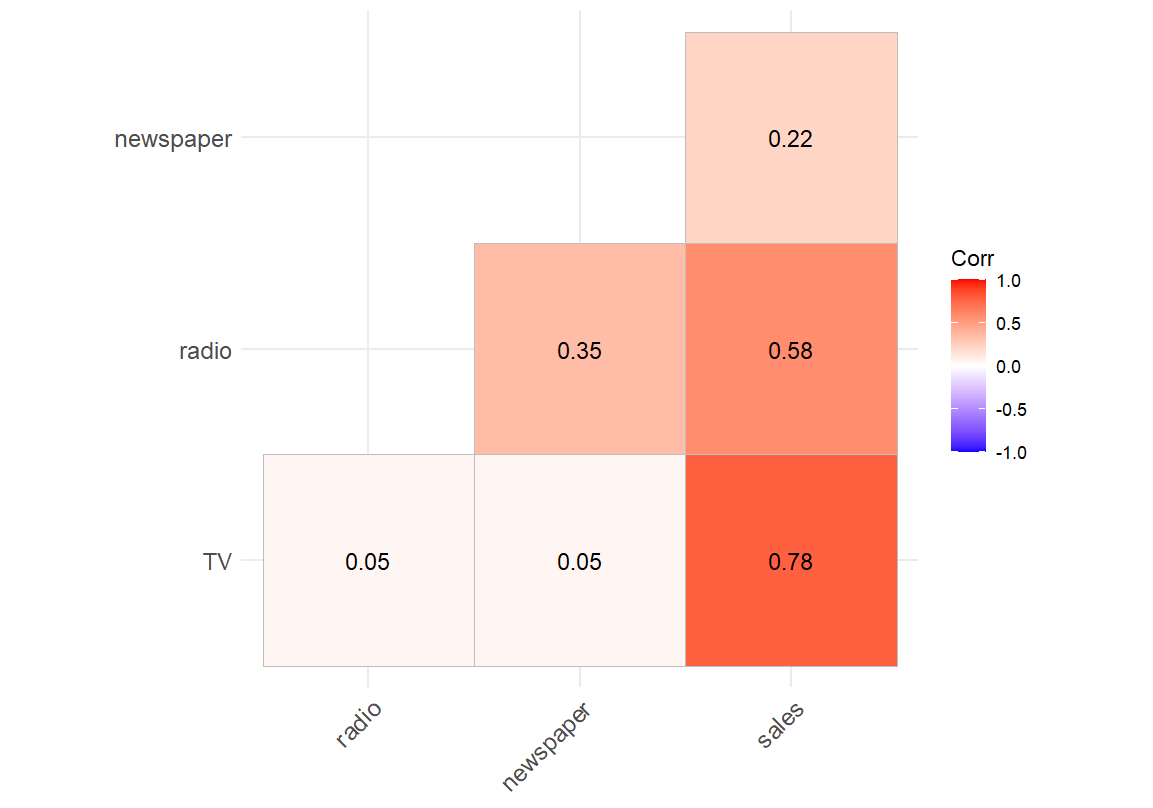
\includegraphics[width=0.7\linewidth]{images/correlation.png}
    \caption{Correlation matrix between variables}
    \label{fig:enter-label}
\end{figure}

The code used to perform analysis, as well as its output, can be found in Appendix A and B respectively.


\section{Model Evaluation}

We begin our model evaluation by analyzing the performance of Model 1, which includes all three predictors: TV, radio, and newspaper. Below is the summary table for Model 1:

\subsection{Model 1 (Full Model)}
\begin{itemize}
    \item Predictors: \textbf{TV, radio, and newspaper}
    \item Equation:
    \begin{equation}
        \hat{y} = \beta_0 + \beta_1 TV + \beta_2 radio + \beta_3 newspaper
    \end{equation}
    \item Adjusted $ R^2 $: \textbf{0.8915}
    \item MSE on test set: \textbf{2.08497}
    \item Coefficients and statistical significance:
\end{itemize}

\begin{table}[h]
    \centering
    \begin{tabular}{lcccc}
        \toprule
        Predictor  & Coefficient & Std. Error & t-value & p-value \\
        \midrule
        Intercept  & 2.5064      & 0.3863     & 6.489   & \textbf{1.12e-09} \\
        TV         & 0.0472      & 0.0016     & 29.832  & \textbf{$<$2e-16} \\
        Radio      & 0.1926      & 0.0102     & 18.956  & \textbf{$<$2e-16} \\
        Newspaper  & -0.0017     & 0.0072     & -0.233  & \textbf{0.816} (not significant) \\
        \bottomrule
    \end{tabular}
\end{table}

As observed, the p-value for the newspaper predictor is 0.816, which is much greater than 0.05. This indicates that newspaper advertising does not significantly contribute to predicting sales and should be removed from the model. Consequently, we eliminate the newspaper variable and define our refined model, Model 2, which includes only TV and radio as predictors.

\subsection{Model 2 (Reduced Model using Subset Selection)}
\begin{itemize}
    \item Predictors: \textbf{TV and radio}
    \item Equation:
    \begin{equation}
        \hat{y} = \beta_0 + \beta_1 TV + \beta_2 radio
    \end{equation}
    \item Adjusted $ R^2 $: \textbf{0.8921} (higher than Model 1, despite one fewer predictor)
    \item MSE on test set: \textbf{2.08459} 
    \item Coefficients and statistical significance:
\end{itemize}

\begin{table}[h]
    \centering
    \begin{tabular}{lcccc}
        \toprule
        Predictor  & Coefficient & Std. Error & t-value & p-value \\
        \midrule
        Intercept  & 2.4734      & 0.3584     & 6.902   & \textbf{1.24e-10} \\
        TV         & 0.0472      & 0.0016     & 29.931  & \textbf{$<$2e-16} \\
        Radio      & 0.1919      & 0.0097     & 19.819  & \textbf{$<$2e-16} \\
        \bottomrule
    \end{tabular}
\end{table}
\newpage
To confirm the superiority of Model 2 over Model 1, we compare their performance metrics. The adjusted $R^2$ value for Model 1 is 0.8915, whereas for Model 2, it is 0.8921. Since the adjusted $R^2$ value slightly increases in Model 2, this indicates a better fit by removing the newspaper predictor. Furthermore, the Mean Squared Error (MSE) values for the test set are:

\begin{itemize}
    \item Model 1: $2.08497$
    \item Model 2: $2.08459$
\end{itemize}

Since Model 2 achieves a marginally lower MSE and a higher adjusted $R^2$, we conclude that it is the better model for predicting sales. Therefore, Model 2 is selected as our final model for making predictions.

\subsection{Durbin-Watson Test}
\begin{itemize}
    \item The test for autocorrelation yielded a \textbf{DW statistic of 1.8874} and a \textbf{p-value of 0.2385}.
    \item Conclusion: We fail to reject the null hypothesis, meaning \textbf{no significant autocorrelation in residuals}, which supports model validity.
\end{itemize}

\subsection{Residual Analysis}
\begin{itemize}
    \item \textbf{Histogram and Q-Q plot of residuals} suggest they are approximately normally distributed, though with slight deviation.
    \item \textbf{Residuals vs. Fitted plot} does not show clear heteroscedasticity, meaning variance is fairly constant.
    \item \textbf{Cook’s Distance test for influential points} found several high-leverage points (e.g., indices 3, 6, 26, 36, 76, 77, 92, 118, 127, 131, 179), but they were not removed as their impact was minor.
\end{itemize}

%If preferred paragraph format instead use the commented stuff below

\begin{comment}
    We begin our model evaluation by analyzing the performance of Model 1, which includes all three predictors: TV, radio, and newspaper. The regression equation for this model is given as:
\begin{equation}
\hat{y} = \beta_0 + \beta_1 TV + \beta_2 radio + \beta_3 newspaper
\end{equation}
The adjusted $R^2$ value for Model 1 is 0.8915, indicating a strong fit, while the Mean Squared Error (MSE) on the test set is 2.08497. The coefficients and their statistical significance are presented in the following table:

\begin{table}[h]
    \centering
    \begin{tabular}{lcccc}
        \toprule
        Predictor  & Coefficient & Std. Error & t-value & p-value \\
        \midrule
        Intercept  & 2.5064      & 0.3863     & 6.489   & \textbf{1.12e-09} \\
        TV         & 0.0472      & 0.0016     & 29.832  & \textbf{$<$2e-16} \\
        Radio      & 0.1926      & 0.0102     & 18.956  & \textbf{$<$2e-16} \\
        Newspaper  & -0.0017     & 0.0072     & -0.233  & \textbf{0.816} (not significant) \\
        \bottomrule
    \end{tabular}
\end{table}

From the table, it is evident that the newspaper predictor has a p-value of 0.816, which is much greater than 0.05. This implies that newspaper advertising does not significantly contribute to predicting sales. To improve the model, we remove the newspaper variable and define Model 2, which includes only TV and radio as predictors.

In Model 2, the refined regression equation is:
\begin{equation}
\hat{y} = \beta_0 + \beta_1 TV + \beta_2 radio
\end{equation}
After removing the newspaper variable, the adjusted $R^2$ value increases slightly to 0.8921, demonstrating an improved model fit. The MSE on the test set remains nearly identical at 2.08459. The coefficient estimates and statistical significance for Model 2 are summarized in the table below:

\begin{table}[h]
    \centering
    \begin{tabular}{lcccc}
        \toprule
        Predictor  & Coefficient & Std. Error & t-value & p-value \\
        \midrule
        Intercept  & 2.4734      & 0.3584     & 6.902   & \textbf{1.24e-10} \\
        TV         & 0.0472      & 0.0016     & 29.931  & \textbf{$<$2e-16} \\
        Radio      & 0.1919      & 0.0097     & 19.819  & \textbf{$<$2e-16} \\
        \bottomrule
    \end{tabular}
\end{table}
\newpage
Comparing the two models, Model 2 outperforms Model 1 in terms of adjusted $R^2$, which increases from 0.8915 to 0.8921, suggesting a slightly better fit despite having one fewer predictor. Furthermore, the MSE values for the test set are 2.08497 for Model 1 and 2.08459 for Model 2, indicating an improvement in prediction accuracy. Since Model 2 achieves a marginally lower MSE and a higher adjusted $R^2$, we conclude that it is the superior model for predicting sales.

To ensure the validity of our model, we conducted a Durbin-Watson test to check for autocorrelation in the residuals. The test resulted in a Durbin-Watson statistic of 1.8874 with a p-value of 0.2385. Since the p-value is not significant, we fail to reject the null hypothesis, meaning that there is no significant autocorrelation in the residuals. This confirms the reliability of Model 2.

Additionally, a residual analysis was performed to verify model assumptions. The histogram and Q-Q plot of residuals suggest that they are approximately normally distributed, with slight deviations. The residuals versus fitted values plot does not indicate clear heteroscedasticity, implying that variance remains fairly constant across predictions. Furthermore, Cook’s Distance test identified several high-leverage points, including indices 3, 6, 26, 36, 76, 77, 92, 118, 127, 131, and 179. However, their influence on the model was minor, and thus they were not removed.
\end{comment}

\section{Conclusion}
Overall we saw very strong performance from our final model, with an adjusted $R^2$ value of 0.8962 indicating strong fitting to the testing data. Similarly, we saw a low MSE on testing data of 2.08, indicating accurate predictions when used on testing data. 

However, according to our analysis, we find that our assumption of normal residuals may not completely hold, with our Q-Q residuals showing slight deviation from linear pattern. This means that our data may not be perfectly linear. 

In the future, we may want to consider our model with additional data points in the testing set. As we only had around 200 data points, we were only able to split our data 80-20 testing training, and it may be more beneficial to have a more even split for additional testing data, but that would require having access to more data points.

\begin{thebibliography}{9}

\bibitem{hastie}
Hastie, T. (n.d.). \emph{Advertising.csv} [Dataset]. https://trevorhastie.github.io/ISLR/Advertising.csv

\bibitem{R}
\emph{Multiple Linear regression in R - articles - STHDA}. (2018, October 3). http://www.sthda.com/english/articles/40-regression-analysis/168-multiple-linear-regression-in-r/


\bibitem{advert}
\emph{R: Advertising}. (n.d.). https://search.r-project.org/CRAN/refmans/glmtoolbox/html/advertising.html


\end{thebibliography}

\section{Appendices}

\subsection{Appendix A - Source Code}
\begin{verbatim}
    if (!requireNamespace("car", quietly = TRUE)) {
  install.packages("car")
}

install.packages("tidyverse")
install.packages("caTools")
install.packages("ggcorrplot")



library(car)
library(lmtest)
library(tidyverse)
library(caTools)
library(ggcorrplot)

advertising <- read.csv("Advertising.csv")
str(advertising)
head(advertising, 4)

# Visualize variable distributions
for (col_name in names(advertising)) {
  if (is.numeric(advertising[[col_name]])) {
    hist(advertising[[col_name]],
         main = paste("Histogram of", col_name),
         xlab = col_name)
  }
}


# Find the outlier in newspaper
Q1 <- quantile(advertising$newspaper, 0.25)
Q3 <- quantile(advertising$newspaper, 0.75)
IQR <- Q3 - Q1

lower_bound <- Q1 - 1.5 * IQR
upper_bound <- Q3 + 1.5 * IQR

outlier_indices <- which(advertising$newspaper < lower_bound | advertising$newspaper > upper_bound)

print(paste("Outlier value:", advertising$newspapers[outlier_indices]))
print(paste("Outlier indices:", outlier_indices))
advertising <- advertising[-outlier_indices, ]


# Train test split
set.seed(123)
split <- sample.split(advertising$sales, SplitRatio = 0.8)
train_set <- subset(advertising, split == TRUE)
test_set <- subset(advertising, split == FALSE)
dim(train_set)
dim(test_set)

model1 <- lm(sales ~ TV + radio + newspaper, data = train_set)
summary(model1)
summary(model1)$coefficients

model2 <- lm(sales ~ TV + radio, data = train_set)
summary(model2)
confint(model2)

# hist(residuals(model2), main = "Histogram of Residuals", xlab = "Residuals", col = "lightblue", breaks = 20)
qqnorm(residuals(model2))
qqline(residuals(model2), col = "red", lwd = 2)

par(mfrow = c(2, 2))  # Arrange plots in a 2x2 grid
plot(model2)
par(mfrow = c(1, 1))  # Reset plot layout

dwtest(model2)
# sigma(model2)/mean(marketing$sales)

#find MSE on test set
predictions_model1 <- predict(model1, newdata = test_set)
predictions_model2 <- predict(model2, newdata = test_set)

mse_model1 <- mean((test_set$sales - predictions_model1)^2)
print(paste("MSE for model1:", mse_model1))

mse_model2 <- mean((test_set$sales - predictions_model2)^2)
print(paste("MSE for model2:", mse_model2))


#Cook's distance to remove influential points
cooksD <- cooks.distance(model2)
plot(cooksD,type="b",pch=18,col="red")
influential <- cooksD[(cooksD > (3 * mean(cooksD, na.rm = TRUE)))]
print("Indices of influential points:")
print(names(influential))

#correlation between predictors
reduced_data <- subset(advertising, select=-X)
corr_matrix = round(cor(reduced_data),2)

ggcorrplot(corr_matrix, hc.order = FALSE, type="lower", lab=TRUE)
\end{verbatim}

\subsection{Appendix B - Code Output}

\begin{verbatim}
    > dim(train_set)
[1] 158   5

> dim(test_set)
[1] 40  5

> model1 <- lm(sales ~ TV + radio + newspaper, data = train_set)
> summary(model1)

Call:
lm(formula = sales ~ TV + radio + newspaper, data = train_set)

Residuals:
    Min      1Q  Median      3Q     Max 
-8.5519 -0.9765  0.3005  1.1592  3.2111 

Coefficients:
             Estimate Std. Error t value Pr(>|t|)    
(Intercept)  2.506380   0.386262   6.489 1.12e-09 ***
TV           0.047179   0.001582  29.832  < 2e-16 ***
radio        0.192607   0.010161  18.956  < 2e-16 ***
newspaper   -0.001688   0.007246  -0.233    0.816    
---
Signif. codes:  0 ‘***’ 0.001 ‘**’ 0.01 ‘*’ 0.05 ‘.’ 0.1 ‘ ’ 1

Residual standard error: 1.768 on 154 degrees of freedom
Multiple R-squared:  0.8935,	Adjusted R-squared:  0.8915 
F-statistic: 430.8 on 3 and 154 DF,  p-value: < 2.2e-16

> summary(model1)$coefficients
                Estimate  Std. Error   t value     Pr(>|t|)
(Intercept)  2.506379918 0.386261532  6.488816 1.120510e-09
TV           0.047179293 0.001581523 29.831566 6.971047e-66
radio        0.192606578 0.010160618 18.956187 4.186350e-42
newspaper   -0.001688197 0.007245947 -0.232985 8.160824e-01

> model2 <- lm(sales ~ TV + radio, data = train_set)
> summary(model2)

Call:
lm(formula = sales ~ TV + radio, data = train_set)

Residuals:
    Min      1Q  Median      3Q     Max 
-8.5062 -0.9427  0.3082  1.1914  3.1897 

Coefficients:
            Estimate Std. Error t value Pr(>|t|)    
(Intercept) 2.473445   0.358367   6.902 1.24e-10 ***
TV          0.047167   0.001576  29.931  < 2e-16 ***
radio       0.191912   0.009683  19.819  < 2e-16 ***
---
Signif. codes:  0 ‘***’ 0.001 ‘**’ 0.01 ‘*’ 0.05 ‘.’ 0.1 ‘ ’ 1

Residual standard error: 1.763 on 155 degrees of freedom
Multiple R-squared:  0.8935,	Adjusted R-squared:  0.8921 
F-statistic: 650.2 on 2 and 155 DF,  p-value: < 2.2e-16

> confint(model2)
                 2.5 %     97.5 %
(Intercept) 1.76553196 3.18135798
TV          0.04405435 0.05028018
radio       0.17278341 0.21103991

> dwtest(model2)

	Durbin-Watson test

data:  model2
DW = 1.8874, p-value = 0.2385
alternative hypothesis: true autocorrelation is greater than 0

> print(paste("MSE for model1:", mse_model1))
[1] "MSE for model1: 2.08497017705538"

> print(paste("MSE for model2:", mse_model2))
[1] "MSE for model2: 2.08459311158263"

> print("Indices of influential points:")
[1] "Indices of influential points:"

> print(names(influential))
 [1] "3"   "6"   "26"  "36"  "76"  "77"  "92"  "118" "127" "131" "179"

\end{verbatim}

\end{document}
